In this chapter we will cover the most important things that are needed to implement the application.

\section{Libraries}
While coding the application, there's a need to learn about some libraries.

\subsection{Room}
Room makes it easy to work with application's internal database.
For each entity you want to store in database, you define an entity class, which is just a normal kotlin class with some annotations.
For the simplest entity class, you just need to annotate the whole class with \verb|@Entity| and annotate primary key either with \verb|@PrimaryKey| or with multiple primary keys, you can list them as an argument in \verb|@Entity| annotation.
In order to get objects to and from database, you need DAO classes.
The magic is that you declare abstract methods with annotations, optionally with some SQL syntax and Room implements them for you.
Those methods return either the entities, lists of entities or LiveData instances of entities or lists.\cite{room}

\subsection{LiveData}
LiveData is an observable data structure.
Components of view layer can observe those variables, which means that they can react to content changes.
Under the hood, it's a bit more complex.
If content changes multiple times between the screen refresh rate, the view gets only the latest change.
Before observing, the view passes it's own instance of lifecycle, so the LiveData instance knows, when the view is not active or destroyed, so the LiveData instance can delete the reference to this view and stop updating this observer, because of performance and memory leaks.
One of the best things about this library is, that Room can also return LiveData instances, so each time something from the selected group changes, the view knows about it.\cite{livedata}

\subsection{Retrofit}
Retrofit is a nice android library for making network requests.
The setup is similar to Room DAO classes.
For each API call, you define an abstract method.\cite{retrofit}
It also works very well with OkHttp library, which is different http request library, that among everything supports the basic authentication.

\subsection{Coroutines}
Coroutines are kotlin's way to improve multithreaded programming.
It introduces a new keyword \verb|suspend| that can be written in front of methods.
Methods with the \verb|suspend| keyword can't be called the normal way, but can be called from other \verb|suspend| methods or launched via higher order methods of \verb|CoroutineScope|.

\subsection{WorkManager}
WorkManager library is used to handle services.
Service is a part of an application that can run in background and can be started even when the application is not running.
We will be using this for checking execution statuses.

\subsection{Gson}
Gson makes serializing and deserializing java/kotlin objects really easy.
There are no requirements for the code to change in order to use Gson.
It will be used while transforming incoming network content to objects we can work with.

\subsection{Varvet's QR code scanner}
Google made an API for working with QR codes and Varvet made it even easier.
Varvet made an open source project BarcodeReaderSample and published it under MIT license.\cite{varvet}

\subsection{DraggableView by hyuwah}
Pipeline's components should be freely movable across the canvas while editing the pipeline.
That can be achieved by making some regular view (button or image) movable.
This is often achieved by a lot of unnecessary code and that's why we will be using this library that should make it easy.\cite{draggable}

\section{Interesting logic}
This section will describe some of the more complex internal logic.

\subsection{Undo operations}
There are some undo options in planning.
We want the user to be able to undo pipeline deletion or execution deletion.
Just scheduling the sending of the request doesn't do the trick.
We will be creating and storing marks for every scheduled deletion.
So when the application is killed for some reason before the delete request is sent, we can take marks stored in database and send the delete requests at the another start of the application.
Marks can also be used for filtering pipelines and executions that will be showing to the user.
If user undo the deletion, the mark is deleted and the scheduling of the delete request is cancelled.

%\begin{figure}\centering
%    \begin{minipage}[b]{0.45\textwidth}
%    	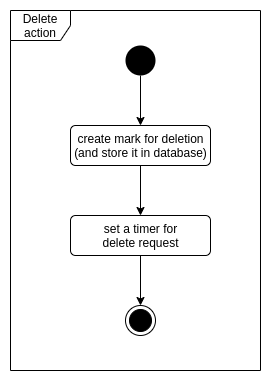
\includegraphics[width=\textwidth]{pics/undo/delete_action.png}
%    	\caption[Delete action]{Delete action}\label{fig:undoDelete}
%    \end{minipage}
%    \begin{minipage}[b]{0.45\textwidth}
%    	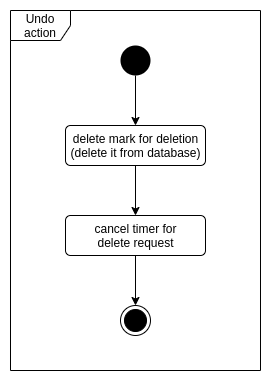
\includegraphics[width=\textwidth]{pics/undo/undo_action.png}
%    	\caption[Undo action]{Undo action}\label{fig:undoUndo}
%    \end{minipage}
%\end{figure}
%\begin{figure}\centering
%    \begin{minipage}[b]{0.45\textwidth}
%    	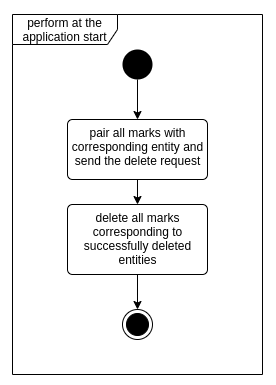
\includegraphics[width=\textwidth]{pics/undo/db_clean.png}
%    	\caption[Finish interrupted delete actions]{Finish interrupted delete actions}\label{fig:undoDbClean}
%    \end{minipage}
%\end{figure}
\begin{figure}\centering
    \begin{minipage}[b]{0.45\textwidth}
    	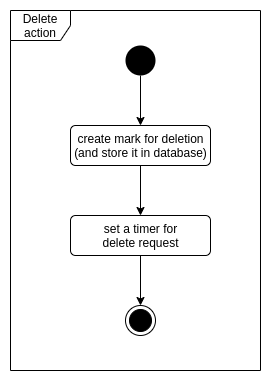
\includegraphics[width=\textwidth]{pics/undo/delete_action.png}
    	\caption[Delete action]{Delete action}\label{fig:undoDelete}
    \end{minipage}
    \begin{minipage}[b]{0.45\textwidth}
    	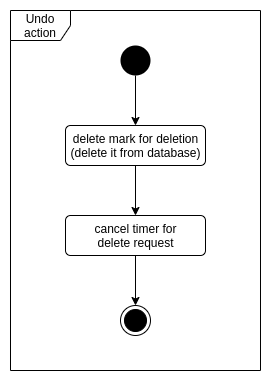
\includegraphics[width=\textwidth]{pics/undo/undo_action.png}
    	\caption[Undo action]{Undo action}\label{fig:undoUndo}
    \end{minipage}
    \begin{minipage}[b]{0.45\textwidth}
    	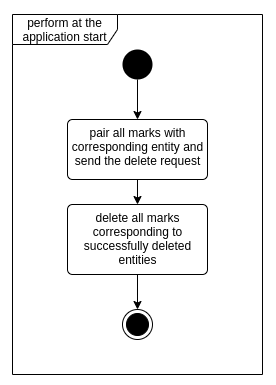
\includegraphics[width=\textwidth]{pics/undo/db_clean.png}
    	\caption[Finish interrupted delete actions]{Finish interrupted delete actions}\label{fig:undoDbClean}
    \end{minipage}
\end{figure}

\subsection{Execution status}
In order to know, when an execution is finished or cancelled, the application has to periodically check for it.
By looking at the duration length of executions from the public demo server, it is obvious that most of them don't surpass ten seconds.
But looking at executions from one private server, they least for hours and some of them even days.
We will be using this checking strategy:
\begin{itemize}
    \item For the first 10 seconds, check every second.
    \item Next 50 seconds, check every 5\textsuperscript{th} second.
    \item Then check once every hour.
\end{itemize}

\section{Tests}
It is a good practise to write special code that can check whenever parts of the application work as intended.
This code is simply called tests.
This is not only useful to test the application parts when they are written, but these tests could be run in future to ensure that possible code changes didn't broke the functionality of previously written parts.

We will be using libraries Hamcrest and MockK.
Hamcrest will be used for matching lists and MockK for mocking.

\subsection{Local unit tests}
These are tests that require only JVM.
They don't need any part of the android framework, so there's no need to run them on an android device, which makes them fast.
Parsing objects from JSON and back can be tested here.

\subsection{Instrumented unit tests}
Instrumented tests require some part of the android framework, so they run in background on an android device.
Previously mentioned library Room requires a part of android framework, so it can be used here.
Repositories can be tested here.

\section{Documentation}
Looking at a code after some time may feel strange and not very intuitive and that's why documentations exist.

\subsection{UI Documentation}
No matter how good the UI is, some users may still struggle with it.
For that case, there will be a UI documentation at the front page of the application's github page, alongside with couple of video tutorials going through previously written use cases.

\subsection{Developer documentation}
In kotlin, there are a documenting type of comment called KDoc.
There is also a plugin called Dokka, that can construct a website based on the KDoc comments, documenting application's code.

It's also a good idea to write a piece of documentation by hand, explaining the internal operations from a greater distance, so other developers can have a more bearable understanding of the application when they follow up on development.